% Author: Hengrui Zhang
% Derived from the ``Northwestern University Thesis Template'' created by Jennifer Klemisch

%%%%%%%%%%%%%%%%%%%%%%%%%%%%%%%%%%%%%%%%%%%%%%%%%%%%
% Document type, global settings, and packages
%%%%%%%%%%%%%%%%%%%%%%%%%%%%%%%%%%%%%%%%%%%%%%%%%%%%

\documentclass[12pt]{report}
\usepackage{graphicx}
\usepackage[letterpaper, margin=1in]{geometry}
\usepackage{setspace}  % use this package to set line spacing as desired
\usepackage{times}  % set Times New Roman as the font
\usepackage[explicit]{titlesec}  % title control and formatting
\usepackage[titles]{tocloft}  % table of contents control and formatting
\usepackage[bookmarks=true, hidelinks]{hyperref}
\usepackage[backend=biber, bibstyle=ieee, url=true]{biblatex}

%\usepackage[bookmarks=true, hidelinks]{hyperref}
\usepackage[page]{appendix}  % for appendices
% \usepackage{rotating}  % for rotated, landscape images
\usepackage[normalem]{ulem}  % for italicized text
\usepackage{pifont}%included by eae1 for checklist 
\usepackage{amssymb} %included by eae1 for checklist pages
\usepackage{fancyhdr} % eae1 added for footer
\usepackage{pdflscape} % eae1 added for landscape code
\usepackage{pythonhighlight}

%%%%%%%%%%%%%%%%
%Caption Settings
%\addto{\captionsenglish}{%
  \renewcommand{\figurename}{Fig.}  
%  \renewcommand{\tablename}{Table}  
%}

%%%%%%%%%%%%%%%%%%%%%%%%%%%%%%%%%%%
% Bibliography settings
%%%%%%%%%%%%%%%%%%%%%%%%%%%%%%%%%%%
%
% Your bibliography file here
\bibliography{references.bib}
%Capitalization of Titles. ASME’s bibliography style requires that titles be in title case. The first letters of principal words are capitalized. This capitalization must be completed when writing the .bib file.
% prevent certain fields in references from printing in the bibliography
\AtEveryBibitem{\clearfield{issn}}
\AtEveryBibitem{\clearlist{issn}}

\AtEveryBibitem{\clearfield{language}}
\AtEveryBibitem{\clearlist{language}}

%\AtEveryBibitem{\clearfield{doi}}
%\AtEveryBibitem{\clearlist{doi}}

%\AtEveryBibitem{\clearfield{url}} %eae1  changed to show url of relevant citations.
%\AtEveryBibitem{\clearlist{url}}

%\AtEveryBibitem{%
%  \ifentrytype{online}
%    {}
%    {\clearfield{urlyear}\clearfield{urlmonth}\clearfield{urlday}}}


%%%%%%%%%%%%%%%%%%%%%%
% Start of Document
%%%%%%%%%%%%%%%%%%%%%%

\begin{document}
\doublespacing  %set line spacing

%%%%%%%%%%%%%%%%%%%%%%%%%%%%%%%%%%%%%
% Title Page
%%%%%%%%%%%%%%%%%%%%%%%%%%%%%%%%%%%%%

%%%%%%%%%%%%%%%%%%%%%%%%%%%%%%%%%%%%%%%%%%%%%%%%%%%%%%%%%
% Edit these lines for your title page.
%%%%%%%%%%%%%%%%%%%%%%%%%%%%%%%%%%%%%%%%%%%%%%%%%%%%%%%%%

\begin{titlepage}
   \begin{center}
 %      \vspace*{cm}

     Cal Poly Humboldt
 School of Engineering\\
Fall 2025 ENGR 326 Computational Methods III \\
Course Instructors: 
       Bonnie Ludka \& 
       Emily Lavrador
       \vspace{3cm}

% Put your title here
% Be sure to include the problem and the solution method 
\textbf{\LARGE Prototype Rotorcraft Service Ceiling Determination with the Runge-Kutta-Fehldberg Method }

       \vspace{1cm}
       \large{ Client: Jason Cowper, Lead Engineer\\
        Organization: Summit Rotorcraft Systems}
            
       \vspace{2cm}
       {\large  Submitted by: Jaxon Cooper}\\
       

\vspace{2cm}
            
            \today

                   \vfill
            
          
\includegraphics[width=0.3\textwidth]{images/spiritSeal_CalPolyHumboldt_fullColor.png}
     
%If you want       \includegraphics[width=0.4\textwidth]{university}
            
          \end{center}
\end{titlepage}
\currentpdfbookmark{Title Page}{titlePage}  %add PDF bookmark for this page

\pagenumbering{roman}
\setcounter{page}{1} % set the page number appropriately

%%%%%%%%%%%%%%%%%%%%%%%%%%%%%%%%%%%%%%%%%%%%%%%%%%%%%%%%%%%%%%%%%

%%%%%%%%%%%%%%%%%%%%%%%%%%%%%%%%%%%%%
% Table of Contents
%%%%%%%%%%%%%%%%%%%%%%%%%%%%%%%%%%%%%

% Format for Table of Contents
\renewcommand{\cftchapdotsep}{\cftdotsep}  %add dot separators
\renewcommand{\cftchapfont}{\bfseries}  %set title font weight
\renewcommand{\cftchappagefont}{}  %set page number font weight
%\renewcommand{\cftchappresnum}{Chapter }
%\renewcommand{\cftchapaftersnum}{:}
%\renewcommand{\cftchapnumwidth}{5em}
\renewcommand{\cftchapafterpnum}{\vskip\baselineskip} %set correct spacing for entries in single space environment
\renewcommand{\cftsecafterpnum}{\vskip\baselineskip}  %set correct spacing for entries in single space environment
\renewcommand{\cftsubsecafterpnum}{\vskip\baselineskip} %set correct spacing for entries in single space environment
\renewcommand{\cftsubsubsecafterpnum}{\vskip\baselineskip} %set correct spacing for entries in single space environment

%format title font size and position (this also applies to list of figures and list of tables)
\titleformat{\chapter}%[display]
{\normalfont\bfseries%\filcenter}
}{\thechapter}{5pt}{\MakeUppercase{#1}}
%\chaptertitlename


\renewcommand\contentsname{Table of Contents}

\begin{singlespace}
\tableofcontents
\end{singlespace}

\currentpdfbookmark{Table of Contents}{TOC}
\clearpage

%%%%%%%%%%%%%%%%%%%%%%%%%%%%%%%%%%%%%
% List of figures and tables if needed
%%%%%%%%%%%%%%%%%%%%%%%%%%%%%%%%%%%%%
 \addcontentsline{toc}{chapter}{List of Figures}
 \begin{singlespace}
 \setlength\cftbeforefigskip{\baselineskip}  %manually set spacing between entries
 \listoffigures
 \end{singlespace}
 BE SURE TO REMOVE THIS TEXT.... You must have at least six (6) different types of non-text content (i.e.photo, table, graph, diagram etc), including at least: 1 \& 2) Two pictures or diagrams of the problem, 3 \& 4) two pictures or diagrams of the solution method  5) one figure or table showing your results, 6) one figure or table showing sensitivity analysis results. 
Of course, you are free to include more than six, but avoid you building out your page length with tons of figures.  Include useful and relevant figures. 
If you want to show a lot of figures but they are not critical for the main 
report, throw them into an appendix. Be sure to include captions and text to support each figure and table, even in the appendix.

 \clearpage

 \addcontentsline{toc}{chapter}{List of Tables}
 \begin{singlespace}
 	\setlength\cftbeforetabskip{\baselineskip}  %manually set spacing between entries
 	\listoftables
 \end{singlespace}
 \clearpage


%%%%%%%%%%%%%%%%%%%%%%%%%%%%
% MAIN TEXT
%%%%%%%%%%%%%%%%%%%%%%%%%%%%

%%%%%%%%%%%%%%%%%%%%%%
% formatting
%%%%%%%%%%%%%%%%%%%%%%

\pagestyle{fancy} %eae1 for footers
\fancyhf{}
\fancyhead[]{\nouppercase{\rightmark\hfill\leftmark}}
%\fancyhead{} % will clear the headers
\fancyfoot[R]{Cooper, \today}
% start page numbering for main text
\clearpage
% Adjust chapter title formatting
%\titleformat{\chapter}[display]
%{\normalfont\bfseries\filcenter}{\MakeUppercase\chaptertitlename\ \thechapter}{0pt}{\MakeUppercase{#1}}  %spacing between titles
%\titlespacing*{\chapter}
%  {0pt}{0pt}{30pt}	%controls vertical margins on title
  
% Adjust section title formatting
\titleformat{\section}{\normalfont\bfseries}{\thesection}{1em}{#1}

% Adjust subsection title formatting
\titleformat{\subsection}{\normalfont}{\uline{\thesubsection}}{0em}{\uline{\hspace{1em}#1}}

% Adjust subsubsection title formatting
\titleformat{\subsubsection}{\normalfont\itshape}{\thesubsection}{1em}{#1}

%%%%%%%%%%%%%%%%
% Chapters
%%%%%%%%%%%%%%%%

%\pagenumbering{arabic}
% Please include an Executive Summary for your final project:
\chapter*{Executive Summary}
\addcontentsline{toc}{section}{Executive Summary}

Summit Rotorcraft Systems (SRS), a helicopter manufacturer, is in the analysis stage of a new prototype. The analysis is being led by Jason Cowper,
the lead engineer on the prototype team, prior to testing stages. A critical component in the prototype analysis is the confirmation that its
predicted operational performance complies with the rigorous safety policies of the Federal Aviation Administration (FAA).

A primary performance threshold of the rotorcraft that must be measured is its minimum vertical rate of climb (VROC). Maintaining VROC above
this minimum, or critical, value ensures that the rotorcraft can maintain a safe level of maneuvarability. VROC decreases as altitude
increases, which implies that critical VROC is the detemining factor for the maximum safe altitude the rotorcraft can operate at. This
maximum altitude is known as a rotorcraft's service ceiling.

Jason Cowper is requesting a computational model that can predict the service ceiling of the new rotorcraft protoype. This model will
calculate the prototype's service ceiling, as well as the time that will elapse to dynamically approach this service ceiling, named as 
time-to-climb (TTC).

The model will first receive inputs of the protoype helicopter's specifications developed by SRS. It will then utilize known International
Standard Atmosphere (ISA) parameters to calculate density, required turbine power, and available turbine power, all varying with altitude.
It will then use these calculations to determine a steady state VROC which can be utilized for climb dynamics.

The climb dynamics algorithm will be solved by the Runge-Kutta-Fehldberg method to generate a set of altitudes, with corresponding
VROC values, which vary with time. The service ceiling will be determined by finding the altitude that has a corresponding VROC that has
decreased to the critical rate value determined for this rotorcraft. The TTC corresponding with service ceiling is also found from this
service ceiling determination.

The computational model determined a service ceiling, based on prototype specifications, to be a maximum altitude of 5118 meters, or 16791 feet.
The dynamic TTC to approach this service ceiling, is determined to be 24.4 min.

The service ceiling and TTC measurements were observed to be highly sensitive to the variance of sea-level turbine power and rotor size.
Percent differences are identical between variance of power and rotor size.

The resultant service ceiling and TTC are determined to be appropriate performance measurements for the new rotorcraft prototype. It is
recommended to continue with development plans of the prototype using current specifications.


\newpage
% optional: You could include an Acknowledgements section where you acknowledge those that have assisted you. 
\chapter*{Forward}
\addcontentsline{toc}{section}{Forward}

This project was chosen to provide an opportunity to gain more experience in mathematical computations for an aerospace
application. The physical behavior of a rotorcraft, and the ability to create a mathematical model of said behavior, is
a very valuable skill to develop and improve for future work. Dynamic behavior in helicopter climb rate is a very complex
measurement that requires the consideration of many external factors, and this climb dynamics algortihm provides a simplified
behavior model for basic predictions. These predictions can be extremely valuable for future prototype testing.

\newpage
\pagenumbering{arabic}
\setcounter{page}{1} % set the page number appropriately

\chapter{Introduction}
The Introduction Section provides an overview of the problem, with relevant objectives and reasoning for solving.
\section{Overview of the Problem} 
Summit Rotorcraft Systems (SRS) is a helicopter manufacturer developing a new model prototype. This prototype is required to
adhere to the rigorous performance regulations enforced by the Federal Aviation Administration (FAA). A primary performance
measurement that the prototype must satisfy is the minimum, or critical, vertical rate of climb (VROC) requirements. This critical
VROC will be the determining factor for the service ceiling of the rotorcraft. Jason Cowper, the lead engineer of the SRS prototype
team, is requesting a computational model that can calculate the service ceiling of the new rotorcraft.

\section{Objectives} 
The following objectives are addressed in this report:
\begin{enumerate}
    \item \textit{Steady State VROC} Determine steady state VROC as a function of altitude.
    \item \textit{First Order ODEs} Determine first order ODEs from the second order climb dynamics ODE.
    \item \textit{Altitudes and VROCs} Use the Runge-Kutta-Fehldberg method to find altitude and VROC values that change with time.
    \item \textit{Service Ceiling} Determine service ceiling from VROC and altitude results.
    \item \textit{Dynamic TTC} Record the corresponding TTC from elapsed time to reach service ceiling.
\end{enumerate}

\section{Motivation}

The use of this developed computational model is not exclusive to the SRS prototype. The specifications of any helicopter can be used in the
model to predict a unique service ceiling and dynamic TTC. This model is simple enough to efficiently calculate these values in a short time
period, while still being accurate enough for a strong prediction for future live testing.

\chapter{Background} 
This section will introduce the client, the problem situation, relevant literature, and method options.

\section{Client Background}
Jason Cowper is the lead engineer on the prototype team for the Summit Rotorcraft Systems next-generation helicopter.

\section{Problem Situation}
The new helicopter design must adhere to the safety and performance requirements enforced by the FAA. A critical performance measurement
relevant to these requirements is the critical vertical rate of climb (VROC) of the rotorcraft. This VROC is a minimum that the rotorcraft
must never decrease to, so a service ceiling must be determined to ensure this never occurs. Cowper is requesting the development of a
computational model that can determine this altitude threshold, as well as a time-to-climb (TTC) measurement to this altitude.

\section{Case Studies or Relevant Literature}
Much of the fundamental formulas required to solve for induced velocity, required power, available power, and rate of climb are
referenced from the publications of J. Gordon Leishman \cite{helidyn}.

In order to develop realistic prototype rotorcraft specfications, existing light helicopters are referenced to ensure the
prototype is a feasible design. The MD Helicopters MD500 is a prime example of a powerful light duty helicopter that has a
public database of its basic specifications that can be referenced \cite{md500}.

Most fundamental calculations in the computational model require the basic atmospheric parameters published by International
Standard Atmosphere (ISA) \cite{ISA}. These parameters are essential for effective helicopter performance modeling.

\section{Method Options and Justification}
The math model developed for this project, as well as the numerical method used, have been determined to be the most effective
out of all possibilities.

\subsection{Math Model}
The math model utilized in this project is not one that can be altered. Due to the the experimentally calculated parameters and
specifications provided by SRS, there is only one path to determine service ceiling. The required functions of air density,
required power, available power, and induced velocity are essential to make up the math model.

\subsection{Numerical Methods}
The Runge-Kutta-Fehldberg method, or the RK45 method, is the most effective way to solve the second order climb dynamics ODE.
The RK45 method is very effective for non stiff ODEs, due to its stability from adaptive step size \cite{fehlberg,dormandprince}.
Other options, such as the RK4 method, are less reliable due to the fact that they do not have an adaptive step size, which
may result in lower stability.

\chapter{Methods} 
This section will outline the mathematical equations and strategies used to complete the service ceiling and TTC calculations.
The solution approach, math model, and numerical method will all be discussed.

\section{Overview of Approach}
The approach to solve for service ceiling and TTC will begin with the input of rotorcraft specifications and ISA parameters \cite{ISA}.
The second order climb dynamics ODE will then be developed using density, available power, required power, induced velocity,
and steady state VROC, which all vary with altitude. The ODE is then solved with the RK45 method, and the altitude measured at the
critical VROC is obtained for the final result, as well as the corresponding time. A sensitivity analysis is then conducted
to observe service ceiling sensitivity to turboshaft power.

\section{Math Model}

\begin{equation} \label{eq:temp}
    \mathrm T(h)=T_0+Lh
\end{equation}

\noindent where\\
    \indent $T(h)$ is temperature varying with altitude ($K$).\\
    \indent $T_0$ is ISA standard sea level temperature ($K$) \cite{ISA}.\\
    \indent $L$ is ISA standard temperature lapse rate ($\frac{K}{m}$) \cite{ISA}.\\
    \indent $h$ is instantaneous altitude ($m$).

Eq. \ref{eq:temp} calculates temperature as altitude increases.

\begin{equation} \label{eq:density}
    \mathrm \rho(h)=\rho_0(\frac{T(h)}{T_0})^{-\frac{g}{LR}-1}
\end{equation}

\noindent where\\
    \indent $\rho(h)$ is density varying with altitude ($\frac{kg}{m^3}$).\\
    \indent $\rho_0$ is ISA standard sea level density ($\frac{kg}{m^3}$) \cite{ISA}.\\
    \indent $g$ is ISA standard sea level gravity ($\frac{m}{s^2}$) \cite{ISA}.\\
    \indent $R$ is ISA standard specific gas constant for air, $\frac{J}{kgK}$ \cite{ISA}.\\

Eq. \ref{eq:density} calculates density as altitude increases, utilizing ISA measurements to ensure an accurate density
measurement.

\begin{equation} \label{eq:vi}
    \mathrm v_i(h)=\sqrt{\frac{W}{2A\rho(h)}}
\end{equation}

\noindent where\\
    \indent $v_i(h)$ is hover induced velocity ($\frac{m}{s}$) \cite{helidyn}.\\
    \indent $W$ is the maximum gross weight of the rotorcraft ($N$).\\
    \indent $A$ is the rotorcraft rotor disk area ($m^2$).\\

Eq. \ref{eq:vi} determines induced velocity from a hover.

\begin{equation} \label{eq:P_a}
    P_a(h)=\eta P_{SL}(\frac{\rho(h)}{\rho_0})^\alpha
\end{equation}

\noindent where\\
    \indent $P_a(h)$ is available turboshaft power ($W$) \cite{helidyn}.\\
    \indent $\eta$ is mechanical efficiency.\\
    \indent $P_{SL}$ is sea level turboshaft power ($W$).\\
    \indent $\alpha$ is the turboshaft density exponent.\\

Eq. \ref{eq:P_a} determines the total available turboshaft power for flight. Mechanical efficiency $\eta$ is a measurement
calculated by SRS from prototype simulation. Turboshaft density exponent $\alpha$ is a measurement of how sensitive
turboshaft power output is to changes in air density \cite{helidyn}. This exponent has been provided by SRS.

\begin{equation} \label{eq:P_r}
    \mathrm P_r(h)=p_fWv_i(h)
\end{equation}

\noindent where\\
    \indent $P_r(h)$ is required turboshaft power ($W$) \cite{helidyn}.\\
    \indent $p_f$ is the induced power factor.\\

Eq. \ref{eq:P_r} determines required turboshaft power to maintain a hover. Induced power factor $p_f$ indicates the extra turboshaft
power needed to overcome drag produced from thrust \cite{helidyn}.

\begin{equation} \label{eq:roc}
    \mathrm v_{ss}(h)=\frac{P_a(h)-P_r(h)}{W}
\end{equation}

\noindent where\\
    \indent $v_{ss}$ is steady state vertical rate of climb ($\frac{m}{s}$).\\

Eq. \ref{eq:roc} determines steadt state vertical rate of climb, which depends on excess turboshaft power.

\begin{equation} \label{eq:ode}
    \mathrm \tau\frac{d^{2}h}{dt^{2}}+\frac{dh}{dt}=v_{ss}(h)
\end{equation}

\noindent where\\
    \indent $\tau$ is the time constant for lag in vertical speed response ($s$).\\
    \indent $\frac{d^2h}{dt^2}$ is vertical climb acceleration ($\frac{m}{s^2}$).\\
    \indent $\frac{dh}{dt}$ is vertical rate of climb ($\frac{m}{s}$).\\

Eq. \ref{eq:ode} is the second order differential equation that must be solved to determine service ceiling and TTC. Time constant
$\tau$ is an experimentally calculated value, measured from prototype simulation.

\section{Numerical Method}

\begin{equation} \label{eq:RK4}
\mathrm y_{i+1} = y_i+(\frac{37}{387}k_1+\frac{250}{621}k_3+\frac{125}{594}k_4+\frac{512}{1771}k_6)h
\end{equation}

\begin{equation} \label{eq:RK5}
\mathrm y_{i+1} = y_i+(\frac{2825}{27648}k_1+\frac{18575}{48384}k_3+\frac{13525}{55296}k_4+\frac{277}{14336}k_5+\frac{1}{4}k_6)h
\end{equation}

\noindent where\\
\indent $y_i$ is the function evaluation at interval $i$\\
\indent $k_i$ is the slope along each interval $i$\\
\indent $h$ is the step size\\

The numerical method used in this project is the Runge-Kutta-Fehldberg method, also known as RK45. This method solves the ODE
using Eq. \ref{eq:RK5}, and the error is found by finding the difference between this solution and the solution using
Eq. \ref{eq:RK4}. The value of each $k$ coefficient is unique. 

\begin{equation} \label{eq:k1}
\mathrm k_1=f(x_i,y_i)
\end{equation}

\begin{equation} \label{eq:k2}
\mathrm k_2=f(x_i+\frac{1}{5}h,y_i+\frac{1}{5}k_1h)
\end{equation}

\begin{equation} \label{eq:k3}
\mathrm k_3=f(x_i+\frac{3}{10}h,y_i+\frac{3}{40}k_1h+\frac{9}{40}k_2h)
\end{equation}

\begin{equation} \label{eq:k4}
\mathrm k_4=f(x_i+\frac{3}{5}h,y_i+\frac{3}{10}k_1h-\frac{9}{10}k_2h+\frac{6}{5}k_3h)
\end{equation}

\begin{equation} \label{eq:k5}
\mathrm k_5=f(x_i+h,y_i-\frac{11}{54}k_1h+\frac{5}{2}k_2h-\frac{70}{27}k_3h+\frac{35}{27}k_4h)
\end{equation}

\begin{equation} \label{eq:k6}
\mathrm k_6=f(x_i+\frac{7}{8}h,y_i=\frac{1631}{55296}k_1h+\frac{175}{512}k_2h+\frac{575}{13824}k_3h+\frac{44275}{110592}k_4h+\frac{253}{4096}k_5h)
\end{equation}

\noindent Eq. \ref{eq:k1} through Eq. \ref{eq:k6} expand each $k$ value to define the terms used in the RK45 method. The ODEs
will be solved over a range of time values to generate a list of data points. These data points encompass a range of position as
well as velocity for each ODE.

\section{Sensitivity Analysis Methodology}

The purpose of the sensitivity analysis conducted for the rotorcraft prototype is to observe changes in surface ceiling and TTC 
when the turboshaft engine power rating is changed. This knowledge is important for the determination of the final turboshaft
engine choice for the rotorcraft design.

The power rating of the turboshaft engine will be increased and decreased at a steady rate to observe fluctuation in surface
ceiling and TTC. Oberving a linear or non-linear change will be essential in limiting any changes in the current engine rating.

\chapter{Application} 
In this section you will report the values of the data required to complete the analysis. Be sure to cite the source of all data and report all units.  Feel free to update the subsection headers below to reflect your project context. In this section you will address the following questions
\begin{itemize}
\item  What were your data needs?
    \item  How did you gather data?
    \item  What data collection issues/constraints did you have?
    \item  How reliable are your data sources?
\end{itemize}
\section{Math Model Parameters and Values}
You may want to use tables to present your parameter values. 

Table~\ref{table:assembly} and Table~\ref{tab:HorizTab} are example tables. Try to not argue with \LaTeX when \LaTeX decides where to put your figures and tables. 
 Usually \LaTeX puts them in a reasonable place. You can use [b] to put the table or figure at the bottom of a page. 
\begin{table}
\caption{An example table}
\label{table:assembly}
\centering
\renewcommand{\arraystretch}{1.25}
\begin{tabular}{l l} % 2 columns that are left justfied
\hline\hline
\multicolumn{1}{c}{Assembly Attribute} &
\multicolumn{1}{c}{Values} \\ % centered text over 
\multicolumn{1}{c}{(1)} &
\multicolumn{1}{c}{(2)} \\
\hline
Number of particles & 4008 \\
Particle sizes & Multiple  \\
Particle size range & $0.45D_{50}^{\:\ast}$ to $1.40D_{50}$ \\
Initial void ratio, $e_{\mathrm{init}}$ & $0.179$ \\
Assembly size & $54D_{50} \times 54D_{50} \times 54D_{50}$ \\
\hline
\multicolumn{2}{l}{$\ast$ $D_{50}$ represents the median particle diameter} \\
\hline\hline
\end{tabular}
\normalsize
\end{table}

\begin{table}[]
    \caption{Another table example}
    \label{tab:HorizTab}
    \centering
\begin{center}
    \begin{tabular}{ | l | l | l | p{5cm} |}
    \hline
    Day & Min Temp & Max Temp & Summary \\ \hline
    Monday & 11C & 22C & A clear day with lots of sunshine.  
    However, the strong breeze will bring down the temperatures. \\ \hline
    Tuesday & 9C & 19C & Cloudy with rain, across many northern regions. Clear spells 
    across most of Scotland and Northern Ireland, 
    but rain reaching the far northwest. \\ \hline
    Wednesday & 10C & 21C & Rain will still linger for the morning. 
    Conditions will improve by early afternoon and continue 
    throughout the evening. \\
    \hline
    \end{tabular}
\end{center}

\end{table}

\section{Numerical Method Parameters and Values}
 You should refer to your code verification appendix here.  If you would like to cite the source of your code, please see this information \hyperlink{https://scipy.org/citing-scipy}{https://scipy.org/citing-scipy}.

\section{Economic Model Parameters and Values  - Required if seeking an A grade on the Project Report}
Be sure to report only your economic model parameter values here, but no results.
\section{Other Physical Parameters and Values - if needed}
Be sure to delete if you do not use this subsection.
\section{Code Outline \& Model Runs }
 Provide an outline/description of how your code works and is organized.  Be sure to cite sources of any libraries that you used. 
 Use a bulleted or numbered list to outline your model runs. Refer to your numerical methods verification appendix here as well as the appendix that contains your code. You may choose to organize your model runs similar to your numbered project objectives.
\chapter{Results \& Discussion}
Provide text here telling the reader what is in the Results \& Discussion Section.  Avoid having headers without text in between.  Organize your results presentation using the list of objectives you developed in the Introduction. Feel free to introduce new headings to help organize your information. 
\section{Results}
Your results to your math model are presented here.
\subsection{Economic Analysis}
Your results to your optional economic analysis are presented here.
\subsection{Sensitivity Analysis}
Your results to your sensitivity analysis are presented here.

Describe the assessment of the sensitivity of the solution to different parameters, and any input and model errors or uncertainties.  This section should include
\begin{itemize}
    \item a summary of the results of the sensitivity analysis. This summary should include specific information such as a report both the percent change in the parameter and the resulting percent change in the dependent variable.  So, for example, you should say that when parameter $A$ was increased by yy percent, the resulting increase in the dependent variable was xx percent.  Be specific and precise about each report. A bulleted list can be used if you have a lot of parameters.
    \item at least one graphic summary of the sensitivity analysis via a figure or table. A single figure is preferred when all parameters can be compared in one figure.  Figure captions should summarize the take home message of the figure - indicating the parameter(s) the dependent variable is most sensitive to.  Make sure that all figures and tables are discussed and referenced from the text.
\end{itemize}
\section{Discussion}
Provide an overview of this section.  Be sure to address the following subsections content.  If possible, organize your results presentation using the list of objectives you developed in the Introduction. Feel free to introduce new headings to help organize your information.
\subsection{Results}
Discuss your results.
After reporting the results of the program runs with text and figures in the Results Section, this section discusses and interprets the results, while referring to the presented data. No new results should be presented in this section. 


\subsection{Economic Analysis}
Discuss your optional economic analysis.
\subsection{Sensitivity Analysis}
Discuss your sensitivity analysis.

The results of the sensitivity analysis are discussed and interpreted in detail while referring to the presented data. For example, for a given percent change in a parameter value, the percent change in the recommended value or result is discussed and interpreted so that the parameter values or initial conditions are identified that make the most impact on the dependent variable.  No new sensitivity results should be presented in this section.


\subsection{Sources of Error}
Discuss your sources of error.
There are multiple sources of error and each should be discussed.
\begin{enumerate}
    \item Limitations of the math model
    \item Parameter estimation
    \item Numerical methods have truncation error so discuss the error associated with your numerical methods. 
    \item Any computation has round off error.  Round off error is increased with smaller step sized. 
\end{enumerate}


\subsection{Recommendations}
The recommendations should be informed by the sensitivity analysis and the sources of error discussion. 

Present this info as a carefully introduced bulleted list.

\begin{itemize}

\item Recommendations based on Results are presented - usually "answering the question" and likely repeated from the Results section.
\item Recommendations from the sensitivity analysis are discussed - likely repeated Sensitivity Analysis section. 
\item Recommendations can arise from sources of error and would be repeated here.
\item These recommendations also reported in the conclusion and can be copied and pasted.

\end{itemize}   



The entire Results and Discussion section should be at least four pages (including figures and tables).

It is important to differentiate between reporting the Results and interpreting them in the Discussion. Results are just that—the output of the program. The results should be presented graphically in addition to in text and tables. Think about how your results are best conveyed in a non-text-based manner. Also, please make sure your visuals are crisp and clear.  A common error is to identify the most sensitive parameter in the Results Section. This interpretation of the sensitivity results should occur in the Discussion Section. 

When you interpret the results, you can discuss the program that produced the results, the main results and the sensitivity analysis results, and the implication of the sensitivity analysis output on the report’s conclusions. Feel free to discuss any surprises or unexpected outcomes, or to convey that the results  were as anticipated (if that is the case). 

Below are questions this section should address:
\begin{itemize}
    \item Did the approach you took provide results? 
\item What were the results of applying the methodology to the problem?
\item Can you break down the results, with numerical, graphical, or table info to make it more understandable for another engineer?
\item  Can you discuss each table and figure sufficiently so that another engineer can understand it? 
\item How did you assess the sensitivity of the solution to different parameters, and any other errors or uncertainties?
\end{itemize}



\chapter{Conclusions \& Recommendations}

Provide text here telling the reader what is in the Results \& Discussion Section.  Avoid having headers without text in between. 
\section{Conclusions}
Present conclusions here.

The main results as well as the sensitivity analysis are summarized in the Conclusion section as well as Results and Discussion sections because sometimes your reader "just wants to find the answer."
\begin{itemize}
    \item Provide a brief summary of what you have said/made in the whole report
    \item Address the objectives you gave in the introduction—were they met? Why (not)?  It is fine to completely copy and past them as a list here.
\end{itemize}
\section{Recommendations}
Present recommendations here.   Give recommendations if applicable, using a separate paragraph and a bulleted list.  Indicate how the sensitivity analysis informs these recommendations.  You can copy and paste your recommendations from the Recommendations Section.

The entire Conclusions \& Recommendations Section should be one to two pages.

Your conclusions must reflect and respond to the Objectives you established in the Introduction.  Additionally, you must have recommendations for your client going forward. Remember, this section may be the only section that is read by your client.  No new information should be presented in this section.  All conclusions and recommendations should have been presented with context in the Results and Discussion section. 

Below are questions you should address in this section.
\begin{itemize}
    \item  Could you summarize the whole report in a nutshell?
\item Did you adequately address the objectives you gave in the introduction?
\item What were the final technical achievements?
\item Do you have any recommendations? Could have a subheading here to highlight these for the inpatient reader.
\item How did the Sensitivity Analysis inform the conclusion and recommendations?
\end{itemize}
%\section{References}






\pagebreak
% the following section should be removed for the final document
%\section{References} 
Be sure to use high quality references.  Some references should be from peer reviewed journals. Others can be from government documents that outline standards or similar information.  Avoid references to sources that are affiliated with commercial or political organizations unless you have a good reason. For example if you are pricing parts, a .com source would be reasonable.  If your client is from an environmental non-profit, then it would make sense to cite their work. 

One-to-one correspondence. Every reference listed must be cited in the text.  Every citation that meets ASCE requirements, should be listed in references.  When mistakes are made with citations or references, the document becomes less professional and less credible - even verging on dishonest. 

Sometimes, in order to make your scenario work, you might decide to have a fictitious citation and reference.  Be sure to check in with you instructor and be sure to put the word fictitious in your reference.

% Here's the list of references:
\raggedright
%%%%%%%%%%%%%%%%
% References
%%%%%%%%%%%%%%%%
\begin{singlespace}  % use single-line spacing for multi-line text within a single reference
	\setlength\bibitemsep{\baselineskip}  %manually set separataion betwen items in bibliography to double space
	\printbibliography[title={References}]
\end{singlespace}

\addcontentsline{toc}{chapter}{References}  %add References section to Table of Contents
 \label{section:references}

%%%%%%%%%%%%%%%%
% Appendices if applicable
%%%%%%%%%%%%%%%%
% Use package `appendix`

%
%
% Now we start the Appendixes, with the new section name, "Appendix", and a 
%  new counter, "I", "II", etc.
\begin{appendices}

%Some Table of Contents entry formatting
\addtocontents{toc}{\protect\renewcommand{\protect\cftchappresnum}{\appendixname\space}}
\addtocontents{toc}{\protect\renewcommand{\protect\cftchapnumwidth}{6em}}

%Begin individual appendices, separated as chapters
%\appendix
\chapter{Appendices}
%These two commands change the figure and table numbering within the appendix. 
\counterwithin{figure}{section}
\counterwithin{table}{section}

%remove this section
Appendices must be included for 
\begin{itemize}
    \item Program Verification - this section should report how the code was verified and report the percent difference between the best known solution and the solution obtained by the code.  If a different problem was used to verify the code, then that problem should be explained.
    \item Additional data, tables or figures as needed.  Only include this appendix (as always) if you refer to this information in the main document (e.g. Additional explanatory figures are included in Appendix . . .”  Be sure to include text in this appendix, and not just figures and tables etc.  All figures and tables throughout the document must have captions. 
    \item Program code - this section should be the final Appendix.
    \end{itemize}
\section{Address requirements of all technical communication of the SOE at CPH}
Remember the requirements of all technical communication in the Cal Poly School of Engineering - from the syllabus.
\begin{itemize}
    \item All tables must have a table header above the table and all figures must have a figure caption 
below the figure. 
\item Table headings and figure captions should be numbered in the order in which they appear in 
your report. (Thank you LaTeX!)
\item Figures must have only ONE caption – remove the title at the top that EXCEL generates. 
\item All graphs must have axes labeled with units. 
\item Use superscript and subscript fonts when appropriate. Do not use \^ or \_ to denote superscript 
(\^) or subscript (\_) 
\item Equations should be created using an equation editor. (Thank you LaTeX!)
\item When writing decimal values include the leading zero, it helps prevent misreading the value. 
Example: preferred- 0.33 cm; not preferred- .33 cm 
\item All figures must have high quality resolution - no fuzzy figures. 
\end{itemize}
Appendices can be included for 
\begin{itemize}
    \item Additional mathematics
    \item Raw data
    \item Notation
    \item Supplemental information
\end{itemize}

\chapter{Program Verification}
\label{App:Program Verification}
\section{Example Appendix Figure}
Be sure to refer to all figures with in the document.  Figure~\ref{fig:gwgrid1} demonstrates how figure numbering changes for figures in the appendices.
\begin{figure}[] % can put b in [] for bottom
    \centering
    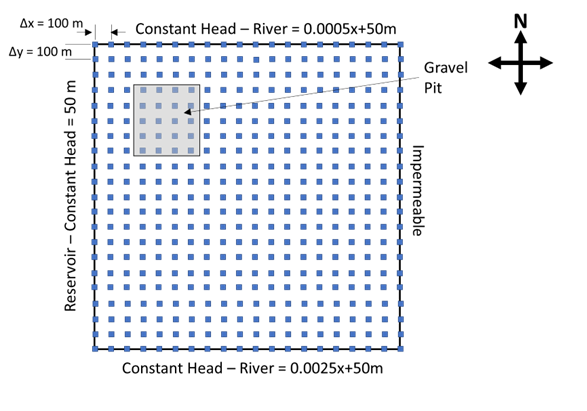
\includegraphics{images/GWgrid.png}
    \caption{Second example of a figure. \protect \cite{anderson2015applied}.}
    \label{fig:gwgrid1}
\end{figure}

\begin{landscape}  % code is presented in landscape
\thispagestyle{empty} %takes footer off first page, but not rest of appendix

\chapter{Program Source Code}
\label{App:Program Source Code}
%or look up other fontsizes to be larger or smaller
%[basicstyle=\footnotesize] %or \small or \tiny etc.

%\begin{lstlisting}[basicstyle=\footnotesize] 
\begin{python}
    print("hello world")
    ##lots of great comments
    ##well structured code
    ##end program example
\end{python}

Or you can input your code from  in an external file but you must edit the file to start and end with the following commands as I did in the file TinyCode.py
\begin{python}
    
\end{python}

\input{TinyCode.py}

    

% you can change the size of the font in a listing by changing the basicstyle from ttfamily to tiny, footnotsize etc  Do a search on ttfamily and you will be all set.
% The following code is in the top of this file where you can change the language and the font size
%\lstset{
%    language=Fortran,
%    language=Python,
%    basicstyle=\ttfamily
%}
\end{landscape}
\end{appendices}
\end{document}